\section{Concept of LEM Simulation Platform}
To start off, this section brings together the previous sections \ref{sec:about_blockchain} and \ref{sec:btm},
and explains how they interact to implement a simulation of a local energy market, which are introduced in section \ref{sec:lem}.
Moreover, this section gives an example for a linear programming problem in terms of energy efficient demand side management of households. 

First, in the presented market mechanism in section \ref{sec:btm}, independent, self-interested agents trading bundled resources
in a double-auction market. 
In case of the developed open-blockchain based LEM simulation, the agents of the \textit{BTM} respresent households. 
These households are trading independently and self-interested bundles of energy resources 
to minimize the monetary expense through optimally scheduling the operation and energy consumption 
of all energy consuming appliances.

Next, blockchain is introduced as the applied ICT of the developed LEM simulation. 
As already mentioned earlier, the implementation of LEM needs 
local distributed control and management techniques, which can addressed by the blockchain technology.
This implies that the respective households submit and receive all relevant data, informations and payments via a blockchain. 
Moreover, the double-auction market which enables households to trade their energy bundles, is operated by a dealer.
In turn, the dealer is implemented by a smart contract, which are introduced in section \ref{sec:smart_contract}, and a conventional software client. 
The dealers' smart contract contains all relevant information regarding the market mechanism, like submitted orders, trades, 
dealers' inventory and market prices. 
Therefore, the households only need to communicate with the dealers' smart contract. 

\begin{figure}[htbp]
	\centering
	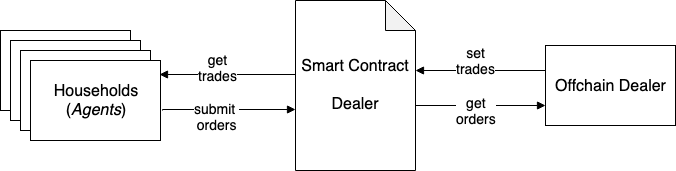
\includegraphics[width=.7\linewidth]{./figures/concept_lem.png}
	\caption{Simplified presentation of the applied communication}
	\label{figure:concept_lem}
\end{figure}

With reference to figure \ref{figure:concept_lem}, the households submit their orders to the dealers' smart contract.  
Afterwards, the dealers' conventional software client, designated as \textit{offchain dealer} in the figure, fetches all existing orders contained in the smart contract
and solves the \text{market matching problem}, which is introduced in section \ref{sec:market_clearing_mechanism}.
Secondly, the \textit{offchain dealer} sets the trades of the settled orders and the new market prices in the smart contract. 
Finally, the households get their respective trades from the dealers' smart contract. 

\begin{comment}

# CONTENT

- Einführung, dass alle bisher vorgestellten Konzepte nun zusammenkommen
- Nähere Erläuterung der Blockchain als ICT. 
- Erklären, dass die Agents aus BTM Haushälte darstellen. 
- Subsection über demand side management der Haushälte einführen 




To start with, we explained in section \ref{sec:lem} that local energy markets enable the trading 
of locally generated energy through a market platform, market mechanism and market access for 
small-scale prosumer and consumer. 
In addition, we presented in section \ref{sec:components_of_local_energy_markets} 
a market mechanism as one of seven core components for a efficient operation of blockchain-based
local energy markets.

Moreover, P2P energy trading in LEM requires advanced communication and data 
exchanges between the different parties, which makes central management and 
operation more and more challenging. The implementation of LEM needs 
local distributed control and management techniques. \shortcite{andoni2019blockchain}. 
\shortciteA{zhang2017review} stated that, P2P energy trading is often
enabled by ICT-based online services. Moreover, \shortciteA{mengelkamp2018designing} explain that 
the new and innovative blockchain technology as an emerging ICT, 
offers new opportunities for decentralized market designs.
It is designed to enable distributed transactions without 
a central trusted entity.
Accordingly, blockchain can help addressing the challenges faced by 
decentralized energy systems

In the proposed framework by, independent, self-interested
agents trading bundled resources in a double-auction market, which run by a dealer. 
In this case, the dealer replaces the central authority and agents represent distributed
entities

\end{comment}